\documentclass{standalone}
\usepackage{pgfplots}
\usetikzlibrary{shapes.geometric, intersections, calc}
\pgfplotsset{compat=1.7}

\begin{document}
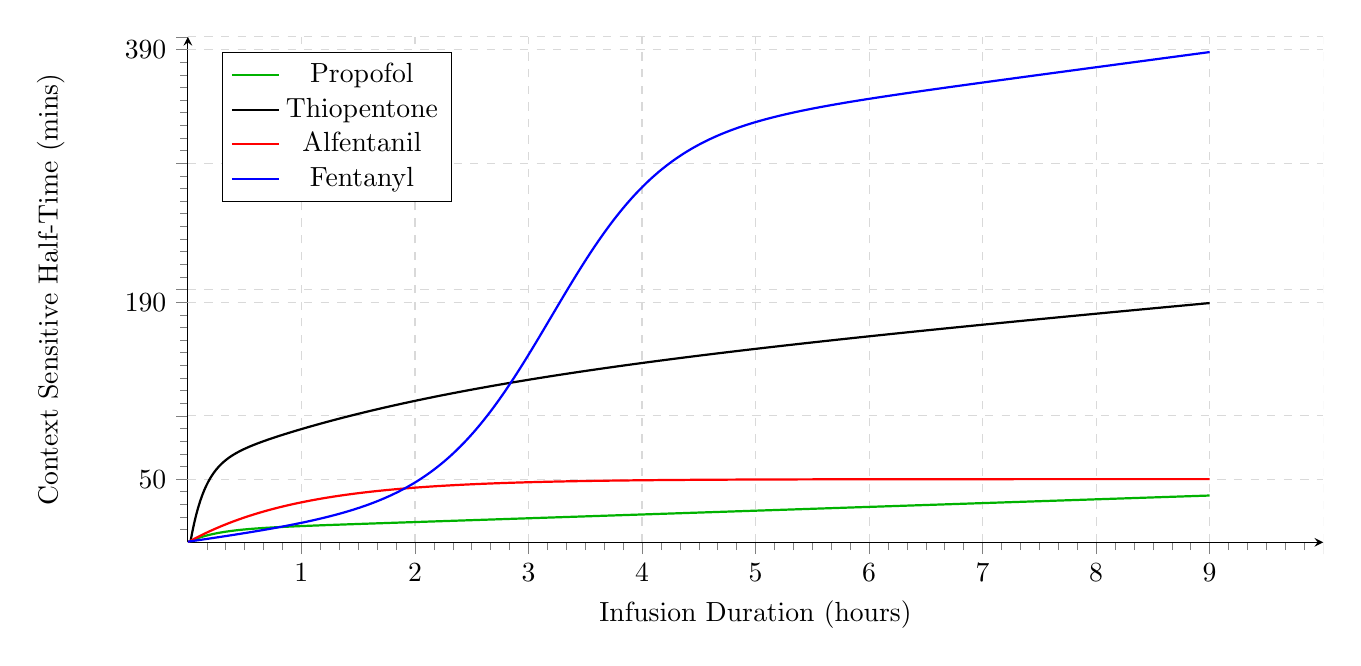
\begin{tikzpicture}[dot/.style={circle,inner sep=1pt,fill,label={#1},name=#1},
 extended line/.style={shorten >=-#1,shorten <=-#1},
 extended line/.default=10cm]

\tikzset{
    myarrow/.style={
        sloped,
        isosceles triangle,
        anchor=apex,
        fill=black,
        inner sep=2pt
    }
}

\makeatletter
\def\parsenode[#1]#2\pgf@nil{%
    \tikzset{label node/.style={#1}}
    \def\nodetext{#2}
}

\tikzset{
    add node at x/.style 2 args={
        name path global=plot line,
        /pgfplots/execute at end plot visualization/.append={
                \begingroup
                \@ifnextchar[{\parsenode}{\parsenode[]}#2\pgf@nil
            \path [name path global = position line #1-1]
                ({axis cs:#1,0}|-{rel axis cs:0,0}) --
                ({axis cs:#1,0}|-{rel axis cs:0,1});
            \path [xshift=1pt, name path global = position line #1-2]
                ({axis cs:#1,0}|-{rel axis cs:0,0}) --
                ({axis cs:#1,0}|-{rel axis cs:0,1});
            \path [
                name intersections={
                    of={plot line and position line #1-1},
                    name=left intersection
                },
                name intersections={
                    of={plot line and position line #1-2},
                    name=right intersection
                },
                label node/.append style={pos=1}
            ] (left intersection-1) -- (right intersection-1)
            node [label node]{\nodetext};
            \endgroup
        }
    },
    add node at y/.style 2 args={
        name path global=plot line,
        /pgfplots/execute at end plot visualization/.append={
                \begingroup
                \@ifnextchar[{\parsenode}{\parsenode[]}#2\pgf@nil
            \path [name path global = position line #1-1]
                ({axis cs:0,#1}-|{rel axis cs:0,0}) --
                ({axis cs:0,#1}-|{rel axis cs:1,1});
            \path [yshift=1pt, name path global = position line #1-2]
                ({axis cs:0,#1}-|{rel axis cs:0,0}) --
                ({axis cs:0,#1}-|{rel axis cs:1,1});
            \path [
                name intersections={
                    of={plot line and position line #1-1},
                    name=left intersection
                },
                name intersections={
                    of={plot line and position line #1-2},
                    name=right intersection
                },
                label node/.append style={pos=1}
            ] (left intersection-1) -- (right intersection-1)
            node [label node] {\nodetext};
            \endgroup
        }
    }
}
\makeatother
    \begin{axis}[
        axis x line=middle,
        axis y line=middle,
        grid = major,
        width=16cm,
        height=8cm,
        grid style={dashed, gray!30},
        xmin=0,     % start the diagram at this x-coordinate
        xmax= 10,    % end   the diagram at this x-coordinate
        ymin= 0,     % start the diagram at this y-coordinate
        ymax= 400,   % end   the diagram at this y-coordinate
        %axis background/.style={fill=white},
    	  x label style={at={(axis description cs:0.5,-0.1)},anchor=north},
	  y label style={at={(axis description cs:-0.1,.5)},rotate=90,anchor=south},
	  xticklabels={1,2,1,2,3,4,5,6,7,8,9},
	 yticklabels={},
	extra y ticks={50, 190, 390},
	extra y tick labels = {50, 190, 390},
	minor x tick num=5,
	minor y tick num=9,
	xlabel near ticks,
        xlabel=Infusion Duration (hours),
        ylabel=Context Sensitive Half-Time (mins),
        tick align=outside,
        enlargelimits=false,
	legend pos = north west]
	\addplot[domain=0:9, black!30!green, thick,samples=500] {10*(1-exp(-4*x)) + 3*x};
	\addlegendentry{Propofol};
	\addplot[domain=0:9, black, thick,samples=500] {70*(1-exp(-8*x)) + 60*(1-exp(-0.5*x)) + 8*x - 12};
	\addlegendentry{Thiopentone};
	\addplot[domain=0:9, red, thick,samples=500] {50*(1-exp(-x))};
	\addlegendentry{Alfentanil};
	\addplot[domain=0:9, blue, thick,samples=500] {280*(1/(1+exp(-2*(x-3.2)))) + 12*x};
	\addlegendentry{Fentanyl};


\end{axis}

\end{tikzpicture} 
\end{document}